\section{Multi-Stage Training for Versatile Locomotion Controllers}\label{sec:training}
Following the construction of the bipedal locomotion controller, our next step in this section involves developing a general framework for training the control policy through reinforcement learning. 
Much like the control structure, this training framework extends beyond a single, specific locomotion skill and is general to various skills.
Such a framework is designed to train the robot in simulation and to transfer to the robot hardware without further fine-tuning. 

\begin{figure}[t]
    \centering
    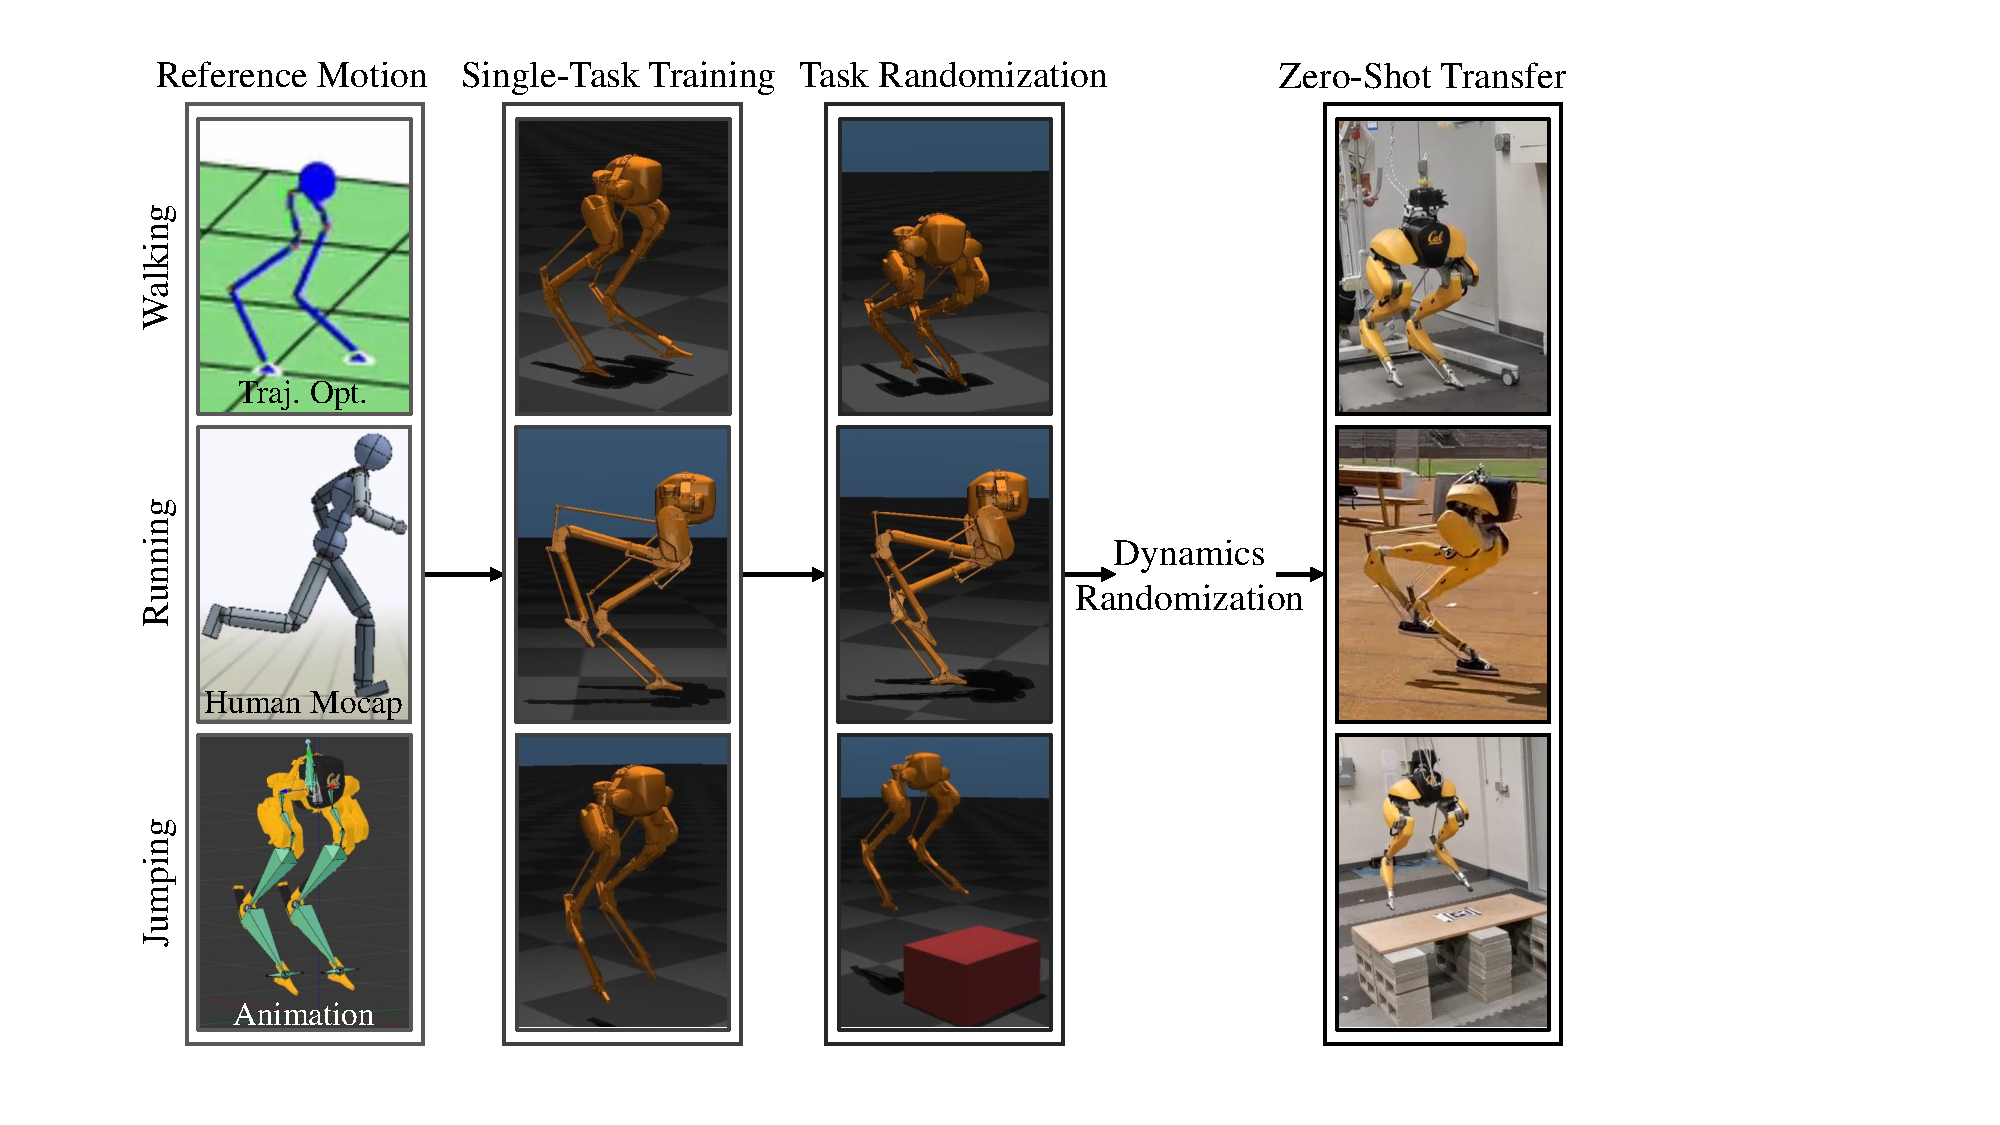
\includegraphics[width=\linewidth]{figures/framework.pdf}
    \caption{The multi-stage training framework to obtain a versatile control policy that can be zero-shot transferred to the real world. It starts with single-task training stage, where the robot is encouraged to mimic a single reference motion with a fixed goal. This is followed by task randomization stage, which expands the range of tasks the robot learns and fosters task generalization resulting in a versatile policy. Once the robot is adept at various locomotion tasks and their transitions, extensive dynamics randomization is incorporated to enhance policy robustness for sim-to-real transfer. This framework is suitable for diverse bipedal locomotion skills, including walking, running, and jumping, and for learning from different sources of skill-specific reference motions such as trajectory optimization, human mocap, and animation.}
    \label{fig:multi_stage_training}
\end{figure}



\subsection{Overview}
It is challenging to train a robot to accomplish diverse tasks through a single control policy via RL. 
This challenge is further compounded when dealing with highly dynamic locomotion maneuvers where the robot has limited support, such as varying running speeds or jumping to different locations. 
In such scenarios, the robot often struggles to learn effectively and may adopt overly conservative strategies, such as merely standing, to circumvent the challenges.
Therefore, we develop a multi-stage training strategy that incorporates a structured curriculum to facilitate the training of versatile locomotion control policies. 
This strategy can be summarized into three stages as shown in Fig.~\ref{fig:multi_stage_training}: (1) single-task training, (2) task randomization, and (3) dynamics randomization.
In the first stage, we concentrate on training the robot to acquire a locomotion skill from scratch, employing a fixed command. 
The primary aim is to equip the robot with the ability to master the skill itself, such as just walking forward, running forward, or jumping in place, while avoiding undesired maneuvering strategies.
In the second stage, we introduce diverse commands to encourage the robot to perform a large variety of tasks using the skill it has acquired to develop a versatile policy.
Following the robot's proficiency in a simple simulation environment, the third stage implements extensive randomization of dynamics parameters in the simulation. 
This process is designed to robustify the policy to ensure a successful zero-shot transfer from simulation to robot hardware.

The design of POMDP, including aspects like reward and episode design, may indeed differ across different stages to serve specific objectives. 
However, the overall multi-stage training scheme remains a general approach to developing different locomotion skills, and as we will see, this method requires only the change of skill-specific reference motion and hyperparameters for learning different skills. 


\paragraph{Combining a Standing Skill} 
Learning a standing skill for the bipedal robot is useful for deployment in the real world, where the robot may need to come to a stop after walking, running, or jumping. 
In the context of the aperiodic jumping skill, the robot learns to maintain a stance pose during the post-landing phase alongside the jumping skill. 
However, this standing skill is not introduced for periodic skills like walking and running. 
To address this gap, in Stage 2, we introduce an additional sub-stage to enable the robot to learn the transition to standing (and back) once it has acquired a versatile policy, with details introduced in Appendix~\ref{appendix:transition_to_stand}.
While previous approaches have explored using separate policies for such a transition, as demonstrated in \cite{crowley2023optimizing}, our work showcases the advantages of having a single policy for transitioning between standing and other locomotion skills. 
This approach can not only realize a rapid transition but also enable the robot to generalize the learned locomotion skill to significantly improve robustness during standing.





\subsection{Reference Motion}
For each locomotion skill, we provide one or a set of reference motions, which provide examples of the type of locomotion maneuvers that the robot is to perform.
As shown in Fig.~\ref{fig:multi_stage_training}, our framework can accommodate diverse sources of reference motion, including reference motions from trajectory optimization, motion capture, and keyframe animations.



\paragraph{Trajectory Optimization}
For the \emph{walking} skill, we leverage the trajectory optimization method to generate a library of reference motions that depict diverse periodic walking gaits based on the robot's full-order dynamics.
The resulting \textit{gait library} is parameterized by the walking commands $[\dot{q}^d_x, \dot{q}^d_y, q^d_z]$ ranging from $[-1.0, -0.3, 0.65]$ to $[1.0, 0.3, 1.0]$, and consists of 1331 different reference motions.
One reference motion is represented by a set of B\'ezier trajectories of each actuated motor with a fixed timespan of the walking period (0.8 seconds). 
A more detailed description of the process for generating the gait library is provided in~\cite[Sec. III-B]{li2020animated} and \citep{hereid2019rapid}. 
Note that we do not consider turning yaw command $q^d_\psi$ when building the reference gait library.  

\begin{table*}[!htp]
\centering
\scriptsize
\caption{The components $\mathbf{r}$ and their respective weights $\mathbf{w}$ in the reward function used for training the bipedal robot across various skills and training stages. A nominal weight vector is provided for different components, with adjustments necessary based on the skill and stage of training, primarily influenced by task diversity (training for single goal versus diverse goals) and the existence of a flight phase. The reward tuning process is relatively streamlined, as only 24 out of 72 reward terms vary across the three different bipedal locomotion skills over multi-stage training. Blank cells indicates no change on the corresponding nominal value.}
\label{tab:reward}
\begin{tabular}{|cccccccc|}
\hline
\multicolumn{1}{|c|}{\multirow{3}{*}{\textbf{Reward Component} $\mathbf{r}$}} &
  \multicolumn{7}{c|}{\textbf{Weight} $\mathbf{w}$} \\ \cline{2-8} 
\multicolumn{1}{|c|}{} &
  \multicolumn{1}{c|}{\multirow{2}{*}{\textbf{Nominal Value}}} &
  \multicolumn{2}{c|}{\textbf{Walking Skill}} &
  \multicolumn{2}{c|}{\textbf{Running Skill}} &
  \multicolumn{2}{c|}{\textbf{Jumping Skill}} \\ \cline{3-8} 
\multicolumn{1}{|c|}{} &
  \multicolumn{1}{c|}{} &
  \multicolumn{1}{c|}{\textbf{Stage 1}} &
  \multicolumn{1}{c|}{\textbf{Stage 2, 3}} &
  \multicolumn{1}{c|}{\textbf{Stage 1}} &
  \multicolumn{1}{c|}{\textbf{Stage 2, 3}} &
  \multicolumn{1}{c|}{\textbf{Stage 1}} &
  \textbf{Stage 2, 3} \\ \hline
\multicolumn{8}{|c|}{\textbf{Motion Tracking}} \\ \hline
\multicolumn{1}{|c|}{Motion position: $r(\mathbf{q}_m, \mathbf{q}^r_m(t))$} &
  \multicolumn{1}{c|}{15} &
  \multicolumn{1}{c|}{} &
  \multicolumn{1}{c|}{} &
  \multicolumn{1}{c|}{} &
  \multicolumn{1}{c|}{} &
  \multicolumn{1}{c|}{} &
  -7.5 \\ \hline
\multicolumn{1}{|c|}{Pelvis height: $r(q_z, q^r_z(t)+\delta_z)$} &
  \multicolumn{1}{c|}{5} &
  \multicolumn{1}{c|}{} &
  \multicolumn{1}{c|}{} &
  \multicolumn{1}{c|}{} &
  \multicolumn{1}{c|}{} &
  \multicolumn{1}{c|}{} &
  -2 \\ \hline
\multicolumn{1}{|c|}{Foot height: $r(\mathbf{e}_z, \mathbf{e}^r_z(t)+\delta_z)$} &
  \multicolumn{1}{c|}{10} &
  \multicolumn{1}{c|}{-7} &
  \multicolumn{1}{c|}{-7} &
  \multicolumn{1}{c|}{} &
  \multicolumn{1}{c|}{} &
  \multicolumn{1}{c|}{} &
  {} \\ \hline
\multicolumn{8}{|c|}{\textbf{Task Completion}} \\ \hline
\multicolumn{1}{|c|}{Pelvis position: $r(q_{x,y}, q^d_{x,y})$} &
  \multicolumn{1}{c|}{7.5} &
  \multicolumn{1}{c|}{-1.5} &
  \multicolumn{1}{c|}{-1.5} &
  \multicolumn{1}{c|}{} &
  \multicolumn{1}{c|}{} &
  \multicolumn{1}{c|}{+5.5} &
  +7.5 \\ \hline
\multicolumn{1}{|c|}{Pelvis velocity: $r(\dot{q}_{x,y}, \dot{q}^d_{x,y})$} &
  \multicolumn{1}{c|}{15} &
  \multicolumn{1}{c|}{} &
  \multicolumn{1}{c|}{} &
  \multicolumn{1}{c|}{} &
  \multicolumn{1}{c|}{} &
  \multicolumn{1}{c|}{-15} &
  -2.5 \\ \hline
\multicolumn{1}{|c|}{Pelvis orientation: $r(\cos(q_{\phi,\theta,\psi}, [0,0,q^d_\psi]), 1)$} &
  \multicolumn{1}{c|}{10} &
  \multicolumn{1}{c|}{-2.5} &
  \multicolumn{1}{c|}{+2.5} &
  \multicolumn{1}{c|}{-5} &
  \multicolumn{1}{c|}{} &
  \multicolumn{1}{c|}{+2.5} &
  {} \\ \hline
\multicolumn{1}{|c|}{Pelvis angular rate: $r(\dot{q}_{\phi,\theta,\psi}, [0,0,\dot{q}^d_\psi])$} &
  \multicolumn{1}{c|}{3} &
  \multicolumn{1}{c|}{} &
  \multicolumn{1}{c|}{} &
  \multicolumn{1}{c|}{} &
  \multicolumn{1}{c|}{+4.5} &
  \multicolumn{1}{c|}{} &
  +7 \\ \hline
\multicolumn{8}{|c|}{\textbf{Smoothing}} \\ \hline
\multicolumn{1}{|c|}{Foot Impact: $r(F_z, 0)$} &
  \multicolumn{1}{c|}{10} &
  \multicolumn{1}{c|}{-7} &
  \multicolumn{1}{c|}{} &
  \multicolumn{1}{c|}{} &
  \multicolumn{1}{c|}{} &
  \multicolumn{1}{c|}{-5} &
  {} \\ \hline
\multicolumn{1}{|c|}{Torque: $r(\bm{\tau}, 0)$} &
  \multicolumn{1}{c|}{3} &
  \multicolumn{1}{c|}{} &
  \multicolumn{1}{c|}{} &
  \multicolumn{1}{c|}{} &
  \multicolumn{1}{c|}{} &
  \multicolumn{1}{c|}{} &
  {} \\ \hline
\multicolumn{1}{|c|}{Motor velocity: $r(\dot{\mathbf{q}}_m, 0)$} &
  \multicolumn{1}{c|}{0} &
  \multicolumn{1}{c|}{} &
  \multicolumn{1}{c|}{} &
  \multicolumn{1}{c|}{} &
  \multicolumn{1}{c|}{+3} &
  \multicolumn{1}{c|}{} &
  {} \\ \hline
\multicolumn{1}{|c|}{Joint acceleration: $r(\ddot{\mathbf{q}}, 0)$} &
  \multicolumn{1}{c|}{3} &
  \multicolumn{1}{c|}{} &
  \multicolumn{1}{c|}{} &
  \multicolumn{1}{c|}{} &
  \multicolumn{1}{c|}{} &
  \multicolumn{1}{c|}{} &
  -3 \\ \hline
\multicolumn{1}{|c|}{Change of action: $r(\mathbf{a}_t, \mathbf{a}_{t+1})$} &
  \multicolumn{1}{c|}{3} &
  \multicolumn{1}{c|}{} &
  \multicolumn{1}{c|}{} &
  \multicolumn{1}{c|}{+2} &
  \multicolumn{1}{c|}{+2} &
  \multicolumn{1}{c|}{-3} &
  +7 \\ \hline
\end{tabular}
\end{table*}


\paragraph{Motion Capture}
The reference motion for the \emph{running} skill is derived from motion capture data collected from a human actor~\citep{sfudatabase}. 
We retargeted the original human motion to the Cassie's morphology using inverse kinematics. 
This process involves matching the motion of key points, such as the pelvis and toes, between the human and the robot. 
More details on the retargeting process is available in ~\cite[Sec. II-B]{li2020animated}. 
Note that we only have \textit{one single} reference motion for periodic running, with an average speed of 3 m/s and foot clearance of around 0.1 m during flight, without lateral or turning movements.
We also retarget \textit{one single} human motion of the transition from running to standing to serve as the reference motion for Cassie to transition between the two behaviors.

\paragraph{Animation}
We provide the reference motion for the \textit{jumping} skill using the animation technique. 
The robot jumping motion is directly hand-crafted in a 3D animation creation suite. 
Similar to running, we only provide a \textit{single} jumping-in-place animation for reference motion, with an apex foot height of 0.5 m, a jumping timespan $T_J=1.66$ seconds, and ending with a stance pose. 
For readers interested in creating animation for bipedal robots, please refer to~\cite{li2020animated}.

Please note that we do not perform trajectory optimization to translate the kinematically feasible reference motion from motion capture or animation to be dynamically feasible for the robot.



\subsection{Reward}\label{subsec:reward}
We now formulate the reward function $r_t$ that the agent receives at each timestep $t$ in order to encourage the robot to perform the desired locomotion skills while completing the desired tasks. 
In this work, the reward $r_t$ the agent receives is the weighted summation of several reward components $\mathbf{r}$, \textit{i.e.}, $r_t = (\mathbf{w}/||\mathbf{w}||_1)^T \mathbf{r}$ with the component vector $\mathbf{r}$ and weight vector $\mathbf{w}$ listed in Table~\ref{tab:reward}.
Each element in $\mathbf{r}$ shares the same format as:
\begin{equation}\label{eq:reward}
    r(\mathbf{u},\mathbf{v}) = \exp({-\alpha||\mathbf{u}-\mathbf{v}||_2}).
\end{equation}\noindent 
By maximizing \eqref{eq:reward}, the robot is incentivized to minimize the distance between two vectors, $\mathbf{u}$ and $\mathbf{v}$. 
In \eqref{eq:reward}, a different scaling factor $\alpha>0$ is introduced in each term to normalize units, resulting in an output range of $(0,1]$.

\subsubsection{Reward Components}
The reward $r_t$ comprises three key terms: (1) motion tracking, (2) task completion, and (3) smoothing. 
Each of these terms consists of several individual reward components, each serving specific objectives, as detailed in Table~\ref{tab:reward}. 

\paragraph{Motion tracking}
The \textit{motion tracking} term is crafted to incentivize the agent to follow the provided reference motion for a specific skill.
This objective is achieved through several components, including the motor position reward $r(\mathbf{q}_m, \mathbf{q}_m^r(t))$, the global pelvis height $r(q_z, q^r_z(t)+\delta_z)$, and the global foot height $r(\mathbf{e}_z, \mathbf{e}^r(t)+\delta_z)$ at each time step.
The addition of $\delta_z$ in the reference vertical displacement takes into account variations in terrain height, such as when the robot encounters changing terrain while running ($\delta_z\coloneqq$ the time-varying terrain height) or when it jumps to different elevations ($\delta_z\coloneqq$ the time-invariant target elevated height). 
There is some privileged environment information used in the reward, such as the robot's global height $q_z$, foot height $\mathbf{e}_z$, or terrain height $\delta_z$. 
These terms provide the robot with better knowledge of the environment and current states during training, but are excluded from the actor's observation. We will frequently see such an exploitation of privileged information in the reward. 

\paragraph{Task completion}
We incorporate a \textit{task completion} term into the reward to ensure that the robot accomplishes the assigned tasks using the acquired locomotion skill. 
Within this term, we motivate the robot to align its movement with the desired velocity and turning rate by including $r(\dot{q}_{x,y}, \dot{q}^d_{x,y})$ and $r(\dot{q}_{\phi,\theta,\psi}, [0,0,\dot{q}^d_{\psi}])$, respectively. 
Additionally, we introduce global pose tracking components $r(q_{x,y}, q^d_{x,y})$ and $r(\cos(q_{\phi,\theta,\psi}-[0,0,q^d_{\psi}]),1)$ in the reward.
Note that for the orientation tracking term, we opt to match $1$ with the $\cos$ of the orientation error within the range of $[-\pi, \pi]$ to prevent singularities when the robot undergoes a transition between $-\pi$ and $\pi$. 
Furthermore, as this work does not consider changes in robot roll and pitch ($q_{\phi, \theta}$), we set $q^d_{\phi, \theta}$ and its rate of change $\dot{q}^d_{\phi, \theta}$ to zero, contributing to the stabilization of the robot's pelvis.
For periodic walking and running skills, the desired velocities $\dot{q}^d_{x,y,\psi}$ are initially provided, and the position terms $q_{x,y,\psi}$ are calculated by integrating the corresponding commands over time. 
Conversely, for aperiodic jumping skills, the desired (time-invariant) landing targets $q_{x,y,\psi}$ are specified first, and average velocity terms are introduced to shape the sparse position reward as $\dot{q}^d_{x,y,\psi}=q^d_{x,y,\psi}/T_J$ where $T_J$ is the jumping timespan.

\paragraph{Smoothing}
Finally, we also add a \textit{smoothing} term to discourage the robot from learning jerky behaviors.
We incentivize the robot to reduce impact forces through $r(F_z,0)$, reduce energy consumption via $r(\bm{\tau},0)$, produce smooth motions by minimizing motor velocities $r(\dot{\mathbf{q}}_m,0)$, damp out joint acceleration $r(\ddot{\mathbf{q}},0)$, and regulate changes in the actions $r(\mathbf{a}_t, \mathbf{a}_{t+1})$.



\subsubsection{Reward Weights}
By employing different choices of weights $\mathbf{w}$, we can emphasize certain reward terms as more critical for the robot's performance while diminishing the significance of others, thereby influencing the robot's acquired maneuvers. 
In this work, despite covering different dynamic locomotion skills and including several training stages for each skill, we demonstrate that the reward components and their associated weight values align with a unified choice (\textit{i.e.}, the nominal value in Table~\ref{tab:reward}) applicable to different skills and stages. 
This homogenization can be achieved with some adjustments in accordance with general principles governing the tuning of specific weight, as detailed in Table~\ref{tab:reward} and introduced below. 

\paragraph{Weights across different stages}
In Stage 1, which involves the initial training of a specific locomotion skill from scratch, our emphasis is placed on training the robot to master the desired skill. As a result, the weight of the \textit{motion tracking} term takes precedence in the reward, encouraging the robot to closely mimic the reference motion.
As the robot becomes proficient in the desired skill, upon entering Stage 2, where the commands are randomized, we can adjust the weight of the \textit{task completion} term to outweigh other terms. 
This adjustment serves to motivate the robot to accomplish different tasks, especially the ones beyond the reference motion, such as executing turning motions in addition to walking, various running and turning speeds that extend beyond the single running reference motion, and various landing targets beyond the single jumping-in-place animation.
To prevent the robot from adopting overly conservative behavior, especially during initial training, the weight of the \textit{smoothing} term remains relatively low. 
As the robot solidifies its locomotion skill, this term can be gradually increased to refine the robot's movements.
But this term is always the least across multiple stages. 


\paragraph{Weights across different skills}
As detailed in Table~\ref{tab:reward}, the variations in the weights among different locomotion skills are generally not substantial, with the primary distinctions arising from the presence of the flight phase in the skill. 
Notably, in skills such as running and jumping, where a significant flight phase is involved, the \textit{motion tracking} term for foot height $r(\mathbf{e}_z, \mathbf{e}^r_z(t) + \delta_z)$ carries a larger weight compared to the walking skill.
Furthermore, to encourage the robot to tackle the challenges caused by the flight phase while deviating from the reference motion to explore diverse tasks, we assign higher weights to the \textit{task completion} term. 
The \textit{smoothing} term largely remains consistent across skills, with some adjustments like the change of action term $r(\mathbf{a}_t, \mathbf{a}_{t+1}$) to strengthen the smoothing of aggressive movements for running and jumping.





\subsection{Episode Design}~\label{subsec:episode_design}

\subsubsection{Unified Approach}
Across all of the diverse locomotion skills and training stages developed in this study, the episode design is consistent and unified. 
The episode duration is set to 2500 timesteps, corresponding to a total timespan of 76 seconds. 
In Stage 2, where variable tasks are introduced, we randomize the command after random time intervals, ranging from 1 second to 15 seconds. 
The specific ranges for uniformly randomized commands for each task are detailed in Table~\ref{tab:command} in Appendix~\ref{appendix:command}. 
Note that we employ a long horizon in an episode to enable the robot to explore more scenarios of transitions among different tasks.

One exception is made for the episode length in the first stage of aperiodic tasks like jumping. 
For such cases, the episode length is adjusted to cover a complete trajectory (\textit{e.g.}, 1.66 seconds for jumping motion), with a significant extension to enable the robot to learn to maintain the last standing pose after landing. 
In this work, the Stage 1 training of jumping employs 750 timesteps (22 seconds).


\subsubsection{Early Termination Conditions}
When training dynamic locomotion skills on bipedal robots, relying solely on reward design could be insufficient. 
The robot might still exhibit undesirable behavior despite achieving suboptimal return, such as maintaining a stance pose without engaging in locomotion because the robot can easily attain part of the reward in this way. 
To address this, in addition to the standard termination conditions, such as the robot falling over ($q_z<0.55$m) or the tarsus joints $q_6^{L/R}$ hitting the ground, we incorporate two additional termination conditions among all skills and stages, as elaborated below. 

\paragraph{Foot height tracking tolerance}
The episode will terminate early if the deviation between the robot's foot height and its reference motion exceeds a threshold $E_e$, \textit{i.e.}, if $|\mathbf{e}_z - \mathbf{e}^r_z(t) - \delta_z| > E_e$. 
This condition is empirically found to be particularly effective in promoting the development of locomotion skills involving flight phases, like running and jumping. 
Without this condition for \textit{motion tracking}, especially during the initial stages of training, the robot tends to remain mostly on the ground.
For skills lacking a flight phase, such as walking, this condition can still be incorporated, although it may not be necessary.


\paragraph{Task completion tolerance}
We underscore the importance of \textit{task completion} to the robot by introducing a condition based on the robot's deviation from the commanded base position and orientation, $|q_{x,y,\psi} - q^d_{x,y,\psi}| > E_t$, with $E_t$ being the acceptable tracking error threshold.
For walking and running, we consistently check this condition to encourage the robot to diminish accumulated tracking errors. 
In the case of jumping, this condition is evaluated after the robot's landing, stimulating the robot to jump to the specified target.

\paragraph{Tolerance across different stages}
The error thresholds $E_e$ and $E_t$ may require adjustments as the training progresses, depending on the robot's proficiency in the desired locomotion skill. 
For instance, the foot height tracking error threshold $E_e$ may start with a tight constraint in the initial stage (Stage 1) and progressively relax in subsequent stages.
Ideally, this condition can be completely removed in the end.
This strategy provides the robot more flexibility in exploring diverse maneuvers in the later stages, surpassing the capabilities of the provided reference motion. 
In contrast, the tracking error threshold $E_t$ can be gradually reduced during training as the robot becomes more skilled in locomotion and can place a stronger emphasis on task completion.
Despite the diversity of skills, we observe a consistent trend in such tolerance adjustments across the multiple training stages.



\subsection{Dynamics Randomization}\label{subsec:domain_rand}
\begin{table}[]
\scriptsize
\caption{The range of dynamics randomization. Introducing simulated external perturbations to the robot's base or incorporating variable terrain is optional but only recommended after the robot has learned to handle general dynamics randomization. However, for highly dynamic skills like aperiodic jumping, external perturbations may not enhance robustness and could stop the robot from learning meaningful maneuvers.}
\centering
\label{tab:randomization}
\begin{tabular}{cc}
\hline
\textbf{Parameters}              & \textbf{Range}                    \\ \hline
\multicolumn{2}{c}{\textbf{Dynamics Randomization (General)}}        \\ \hline
Ground Friction Coefficient             & {[}0.3, 3.0{]}                    \\
Joint Damping Ratio              & {[}0.3, 4.0{]} Nms/rad            \\
Spring Stiffness                 & {[}0.8, 1.2{]} $\times$ default   \\
Link Mass                        & {[}0.5, 1.5{]} $\times$ default   \\
Link Inertia                     & {[}0.7, 1.3{]} $\times$ default   \\
Pelvis (Root) CoM Position   & {[}-0.1, 0.1{]} m in $q_{x,y,z}$  \\
Other Link CoM Position      & {[}-0.05, 0.05{]} m + default     \\
Motor PD Gains                   & {[}0.7, 1.3{]} $\times$ default   \\
Motor Position Noise Mean        & {[}-0.002, 0.002{]} rad           \\
Motor Velocity Noise Mean        & {[}-0.01, 0.01{]} rad/s           \\
Gyro Rotation Noise              & {[}-0.002, 0.002{]} rad           \\
Linear Velocity Estimation Error & {[}-0.04, 0.04{]} m/s             \\
Communication Delay              & {[}0, 0.025{]} s                \\ \hline
\multicolumn{2}{c}{\textbf{External Perturbation (Optional)}}        \\ \hline
Force \& Torque                  & {[}-20, 20{]} N \& {[}-5, 5{]} Nm \\
Elapsed Time Interval (Walking)            & {[}0.1, 3.0{]} s                \\ 
Elapsed Time Interval (Running)            & {[}0.1, 1.0{]} s                \\ \hline
\multicolumn{2}{c}{\textbf{Randomized Terrain (Optional)}}           \\ \hline
Terrain Type                     & Waved, Slopes, Stairs, Steps      \\ \hline
\end{tabular}
\end{table}
As illustrated in Fig.~\ref{fig:multi_stage_training}, in training Stage 3, we introduce randomized dynamics parameters in the simulation environment to train a policy that can stay robust and generalize the acquired locomotion skills to deal with the uncertainty in both \textit{dynamics modeling} and \textit{measurements}. 
The objective of this training is to enable successful transfer from simulation to real-world scenarios where the dynamics parameters are uncertain.
At each episode, dynamics parameters, as detailed in Table~\ref{tab:randomization}, are sampled from their respective uniform distributions. 

Specifically, to address \textit{modeling uncertainty}, we introduce extensive randomization of modeling parameters, including ground friction coefficient, robot joint damping ratio, and mass, inertia, and Center-of-Mass (CoM) position of each link. 
In the case of Cassie, which features passive joints connected by leaf springs, the introduction of $\pm20\%$ randomized stiffness for the leaf springs has been important for successful sim-to-real transfer, particularly for skills like running and jumping that involve substantial compression of the springs.
We also incorporate randomization into the PD gains of the joint-level PD controllers, adding a range of $\pm30\%$ deviation from their default values. 
This randomization is applied independently to each joint-level PD controller. 
This stimulates the diversity in motor responses that can mimic the effects of uncertain motor dynamics seen in real-world scenarios, including motor aging and degradation, which is found effective in facilitating the sim-to-real transfer.

To tackle \textit{measurement uncertainty}, we add a simulated noise to the observable states $\mathbf{o}_t$. 
The noise is modeled as a normal distribution with the mean uniformly sampled from the range specified in Table~\ref{tab:randomization}. 
Please note that, given the reliable sensors like joint encoders and IMU on Cassie's hardware, the range of measurement noise we applied is small. 
However, for robots equipped with lower-quality sensors, a wider simulated noise range may be necessary. 
Additionally, we simulate a communication delay, caused by a zero-order hold, between the policy and the robot's real-time computer, which influences the timing of sending actions and receiving observations. 
For highly dynamic motions, such as jumping and running, the delay plays a significant role in the sim-to-real gap, and the ability to tackle delays during real-time control is critical for stability. 

The randomization strategy mentioned above is applied consistently across various locomotion skills. 
Additionally, we have also investigated the use of other sources of randomization during training. They are randomized perturbation and randomized terrains as detailed below.


\paragraph{Use of Randomized Perturbation}
In our study, we explored the use of randomized external perturbation wrenches applied to the robot's pelvis, hypothesizing that it could create more diverse training scenarios and enhance robustness by deviating the robot from its nominal trajectories. This perturbation (typically being impulse), incorporating forces and torques applied for random durations as specified in Table~\ref{tab:randomization}, can be simulated during training.
However, we find that while this approach can increase the robustness of policies in real-world applications, it introduces complex hyperparameters that are challenging to choose and complicates the training process. For walking, frequent perturbations led to an overemphasis on perturbed scenarios, impairing the robot's performance in normal walking gaits. 
In running, longer perturbations hindered the robot's ability to learn effective gaits. 
As a result, we employed different elapsed time intervals for walking and running, as detailed in Table~\ref{tab:randomization}.
Moreover, in the case of jumping skills or transitions from locomotion to standing, these perturbations proved even more problematic, preventing the robot from acquiring meaningful jumping or standing abilities. Therefore, we chose to exclude external perturbation from the training for both jumping and transition-to-standing skills.


\paragraph{Use of Randomized Terrain}
If the control policy aims to enable the robot to traverse uneven terrain, it is essential to simulate terrain changes during training. 
We developed an algorithm to randomize various types of terrains using parameterized height maps including wave terrain (characterized by sine functions), sloped terrain, monotonic stairs, and random steps, as listed in Table~\ref{tab:randomization}. 
It's important to note that our control policy doesn't incorporate vision, so the robot has to adapt to terrain changes based on its I/O history, making it a more challenging problem.
Terrain randomization is recommended only after the robot has proficiently trained in other dynamics randomization to avoid excessive learning complexity. 
In this study, we introduced terrain randomization for running skills for example. 



\subsection{Training Details}
We develop the simulation of Cassie within the aforementioned environments using MuJoCo based on~\citep{todorov2012mujoco,cassiemj}. 
The training of all control policies is carried out using Proximal Policy Optimization (PPO) developed by~\citep{schulman2017proximal} in simulation.
The control policy (actor) is as described in Sec.~\ref{sec:controller}, with a value function represented by a 2-layered MLP that has access to ground truth observations.
Given the varying complexities of different training stages and skills, the number of training iterations differs across stages and skills. 
The numbers of iterations and other hyperparameters are provided in Table~\ref{tab:num_iter} and Table~\ref{tab:hyperparam_ppo}, respectively, in Appendix~\ref{appendix:hyperparameters}. 

Up to this point, design details of the proposed RL framework for learning versatile, robust, and dynamic bipedal locomotion skills have been introduced. 
We will next proceed to validate several key design components. 
